\newpage
\begin{flushright}
    \textbf{\Large{Ujian Tengah Semester}}
    \subsection*{Tahun 2023}
    \addcontentsline{toc}{subsection}{UTS - 2023}
\end{flushright}
\vspace{0.5cm}
\hrule height 2pt
\vspace{0.5cm}
\begin{center}
    \textbf{\large{MATERI}}
    \begin{enumerate}[leftmargin=*, label={\arabic*}.]
        \item Memahami konsep nilai mutlak
        \item Menyelesaikan pertidaksamaan yang melibatkan nilai mutlak.
        \item Mensketsa grafik fungsi.
        \item Fungsi komposisi dan menentukan domain dan rangenya.
        \item Mencari nilai limit kiri dan nilai limit kanan fungsi.
        \item Mencari nilai limit fungsi di tak hingga.
        \item Menentukan kekontinuan fungsi pada suatu titik.
        \item Menyelesaikan masalah turunan implisit.
        \item Menyelesaikan permasalahan maksimum dan minimum.
    \end{enumerate}
\end{center}
\vspace{0.2cm}
\hrule height 1pt
\vspace{0.5cm}
\begin{center}
    \textbf{\large{SOAL}}
\end{center}
\begin{enumerate}[leftmargin=*, label={\arabic*}.]
\item Misalkan $\ds f(x) = \frac{\sqrt{5}\abs{x}}{x}$ dan $g(x) = -\sqrt{9-x^{2}}$.
\begin{enumerate}[label={\alph*}.]
    \item Tentukanlah domain dan range dari fungsi-fungsi tersebut!
    \item Tentukanlah himpunan penyelesaian dari: $f(x) \geq g(x)$.
\end{enumerate}
\item Diberikan fungsi $f$ dengan $f(x) = \floor{x}^2$.
\begin{enumerate}[label={\alph*}.]
    \item Sketsalah grafik fungsi $f$ tersebut!
    \item Tentukanlah
    \begin{enumerate}[label={\roman*}.]
        \item $f(-1)$
        \item $\ds\lim_{x\to -1^{+}} f(x)$
        \item $\ds\lim_{x\to -1^{-}} f(x)$
        \item $\ds\lim_{x\to -1} f(x)$
    \end{enumerate}
    \item Apakah fungsi $f$ kontinu di $x=-1$? Jelaskanlah!
    \item Jika $f$ tidak kontinu di $x=-1$, apakah ketidakkontinuan tersebut bisa 
    diperbaiki? Jelaskanlah!
\end{enumerate}
\item Carilah persamaan garis singgung dari kurva $(x^2+y^2)^2=(x-y)^2$ di titik $(1,-1)$.
\item Diketahui sebuah fungsi $f$ memenuhi \textbf{semua} kondisi berikut:
\begin{itemize}
    \item $f$ kontinu dimana-mana,
    \item $f(1)=2,f(2)=1,f(4)=4,f(6)=7,f(8)=3$,
    \item $f'(2)=0,f'(4)=1,f'(6)$ dan $f'(8)$ tidak ada,
    
    $f'(x)<0$ untuk $x < 2$ ataua $x>6$, $f'(x)>0$ untuk $2<x<6$,
    \item $f''(4) = 0$, $f''(x)<0$ untuk $4<x<6$ atau $x > 8$,
    
    $f''(x)>0$ untuk $x<4$ atau $6 < x < 8$.
\end{itemize}
\begin{enumerate}[label={\alph*}.]
    \item Di interval manakah fungsi tersebut naik atau turun, cekung ke atas atau 
    ke bawah? Apakah grafik fungsi tersebut mempunyai titik belok 
    (\textit{inflextion point})? Jelaskanlah!
    \item Tentukanlah titik-titik kritis dari fungsi $f$ pada interval 
    $\cintervalo*{1,\infty}$. Kemudian tentukanlah nilai maksimum dan minimum dari fungsi $f$ 
    pada interval tersebut (jika ada)!
    \item Buatlah sketsa grafik fungsi tersebut!
    \item Apakah terdapat bilangan $c$ dalam interval $\cintervalc*{1,6}$ yang memenuhi 
    Teorema Nilai Rata-rata untuk Turunan? Jelaskanlah! Jika ada, tentukanlah \textbf{semua} 
    bilangan $c$ tersebut.
\end{enumerate}
\item Seseorang $(A)$ berdiri di tepi sungai mengamati perahu yang melintas (seperti pada 
gambar di bawah). Asumsikan posisi perahu saat melaju selalu tepat di tengah sungai. Diketahui 
lebar sungai adalah $12$ meter. Jika sudut pengamatan antar $A$ dengan perahu adalah 
$\theta =\frac{\pi}{2}$rad dan kecepatan perubahan sudut $\theta$ adalah $3$rad/detik, berapa 
kecepatan perahu pada saat itu?
\vspace{0.2cm}
\begin{center}
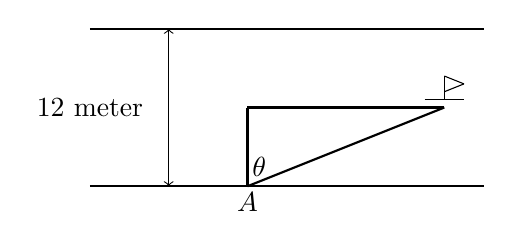
\begin{tikzpicture}
    \draw[thick] (-2,1)--(3,1);
    \draw[thick] (-2,-1)--(3,-1);
    \draw[thin, <->] (-1,-1)--(-1,1);
    \draw[thick] (0,-1)--(0,0);
    \draw[thick] (0,0)--(2.5,0);
    \draw[thick] (0,-1)--(2.5,0);
    \draw[thin] (2.25,0.1)--(2.75,0.1);
    \draw[thin] (2.5,0.1)--(2.5,0.4);
    \draw[thin] (2.75,0.3)--(2.5,0.4);
    \draw[thin] (2.75,0.3)--(2.5,0.2);
    
    \node at (-2,0) {$12$ meter};
    \node at (0.15,-0.75) {$\theta$};
    \node at (0,-1.2) {$A$};
    \end{tikzpicture}
\end{center}
\end{enumerate}
\vspace{0.2cm}
\hrule height 1pt
\vspace{0.5cm}
\begin{center}
    \textbf{\large{PEMBAHASAN}}
\end{center}
\begin{enumerate}[leftmargin=*, label={\arabic*}.]
\item Halo

\end{enumerate}

\begin{center}
    \line(1,0){300}
\end{center}